\documentclass[tikz]{standalone}
\usepackage{pgfplots}
\pgfplotsset{compat=1.9}
\usepackage[dvipsnames]{xcolor}
\usepackage{amsmath}

\definecolor{gray1}{gray}{0.0}
\definecolor{gray2}{gray}{0.4}
\definecolor{gray3}{gray}{0.65}
\definecolor{gray4}{gray}{0.85}

\colorlet{blue95}{ProcessBlue!95!white}
\colorlet{blue90}{ProcessBlue!50!white}
\colorlet{blue85}{ProcessBlue!85!white}
\colorlet{blue80}{ProcessBlue!80!white}

\newcommand{\users}[0]{\ensuremath{\operatorname{\mathcal{U} }}}
\newcommand{\nusers}[0]{\ensuremath{\operatorname{|\users |}}}
\newcommand{\corrupted}[0]{\ensuremath{\operatorname{\Psi }}}
\newcommand{\ncorrupted}[0]{\ensuremath{\operatorname{|\corrupted |}}}
\newcommand{\advg}[0]{\ensuremath{\operatorname{\alpha}}}
\newcommand{\mixes}[0]{\ensuremath{\operatorname{\mathcal{M}}}}
\newcommand{\nmixes}[0]{\ensuremath{\operatorname{|\mixes|}}}

\begin{document}
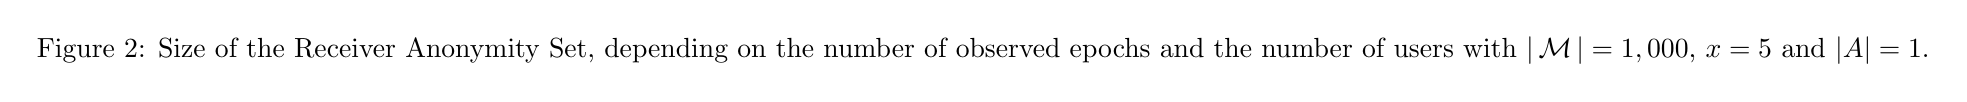
\begin{tikzpicture}
\node{Figure 2: Size of the Receiver Anonymity Set, depending on the number of observed epochs and the number of users with $\nmixes = 1,000$, $x = 5$ and $|A| = 1$.};
\end{tikzpicture}
\begin{tikzpicture}
\begin{axis}[
% axis lines=left,
xlabel={Amount of observed Epochs},
ylabel style={align=center}, 
ylabel={Size of the Receiver Anonymity Set \\(log scale)},
%width=8cm,
height=6cm,
ybar,
xtick={1,2,3},
bar width=7pt,
enlarge x limits= 0.35,
%xmin=0,
xtick distance=0.1,
ymode=log,
ytick={1, 10, 100, 600,6000},
log ticks with fixed point,
    y tick label style={/pgf/number format/1000 sep=\,},
legend image code/.code={
        \draw [#1] (-0.1cm,0.1cm) rectangle (0.3cm,-0.05cm); },
        legend cell align={right},
]
  \addlegendimage{empty legend}
\addlegendentry{\hspace{-1.4cm}\textbf{$\nusers$}}
 \addplot+[
           color=black,
        ]
    table[col sep=comma,header=false,x index=0,y index=5] 
    {data/easis.csv};
    \addlegendentry{1 000 000}
  \addplot+[
           color=gray2,
           ]
    table[col sep=comma,header=false,x index=0,y index=4]
    {data/easis.csv};
    \addlegendentry{100 000}
  \addplot+[
           color=gray3
        ]
    table[col sep=comma,header=false,x index=0,y index=3]
    {data/easis.csv};
       \addlegendentry{50 000}
  \addplot+[
           color=gray4
           ]
    table[col sep=comma,header=false,x index=0,y index=2]
    {data/easis.csv};
    \addlegendentry{10 000}
  %\addplot
 %   table[col sep=comma,header=false,x index=0,y index=1]
 %   {data/easis.csv};
%    \addlegendentry{5 000}

\end{axis}
\end{tikzpicture}
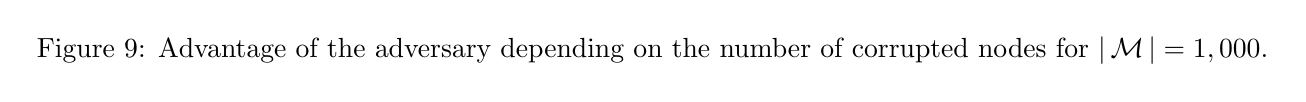
\begin{tikzpicture}
\node{Figure 9: Advantage of the adversary
    depending on the number of corrupted nodes
    for $\nmixes = 1,000$.};
\end{tikzpicture}
\begin{tikzpicture}
  \begin{axis}[
    xlabel={Number of Corrupted Nodes ($\ncorrupted$)},
    ylabel={Advantage ($\advg$)},
    scaled ticks=false,
    width=8cm,
    height=5cm,
    restrict x to domain=1:10,
    restrict y to domain=0:1
    xmin=0,
    ymin=0,
    yticklabel style={/pgf/number format/fixed, /pgf/number format/precision=4},
    xtick={1,2,3,4,5,6,7,8,9,10}
  ]

  \addplot+[ycomb,thick,mark options={black}]
    table[col sep=comma,header=false,x index=0,y index=1]
    {data/lasthop_plot_all_1k.csv};
  \end{axis}
  \end{tikzpicture}
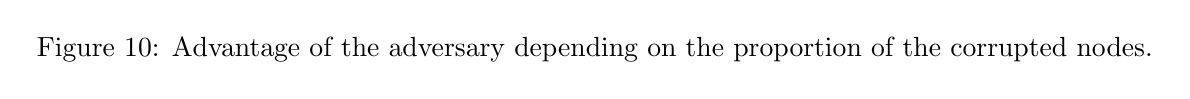
\begin{tikzpicture}
\node{Figure 10: Advantage of the adversary depending
    on the proportion of the corrupted nodes.};
\end{tikzpicture}
    \begin{tikzpicture}
    \begin{axis}[
      % axis lines=left,
      xlabel={Share of Corrupted Nodes $\Bigl(\frac{\corrupted}{\nmixes}\Bigr)$},
      ylabel={Advantage ($\advg$)},
      width=8cm,
      height=5cm,
      xmin=-0,
      ymin=0,
      legend style={at={(0.75,0.2)},anchor=south},
      legend cell align={left},
      legend entries={$\nmixes = 1\,000$, $\nmixes = 100\,000$},
    ]

    \addplot[color=blue,smooth,thick]
      table[col sep=comma,header=false,x index=0,y index=1]
      {data/lasthop_plot_proportion_1k.csv};

    \addplot[only marks,mark size=3pt,mark=triangle*,fill=black]
      table[col sep=comma,header=false,x index=0,y index=4]
      {data/lasthop_plot_ratio_big_steps.csv};
    \end{axis}
  \end{tikzpicture}
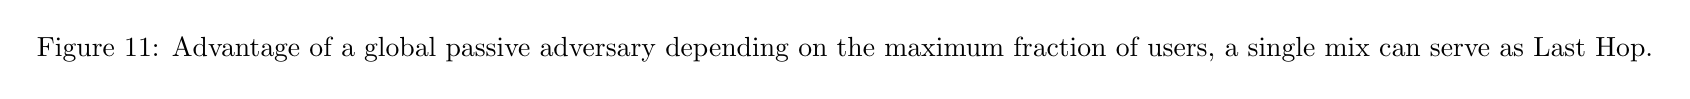
\begin{tikzpicture}
\node{Figure 11: Advantage of a global passive adversary depending on the maximum fraction of users, a single mix can serve as Last Hop.};
\end{tikzpicture}
    \begin{tikzpicture}
  \begin{axis}[
    xlabel={Fraction of Users Allowed on the Same Mix ($\frac{1}{x}$)},
    ylabel={Advantage ($\advg$)},
    scaled ticks=false,
    width=8cm,
    height=5cm,
    restrict x to domain=1:10,
    restrict y to domain=0:1
    xmin=0,
    ymin=0,
    yticklabel style={/pgf/number format/fixed, /pgf/number format/precision=4},
     xtick={1,2,3,4,5,6,7,8,9,10}
  ]

  \addplot+[ycomb,thick,mark options={black}]
    table[col sep=comma,header=false,x index=0,y index=1]
    {data/lasthop_plot_global_passive_10.csv};
  \end{axis}
  \end{tikzpicture}
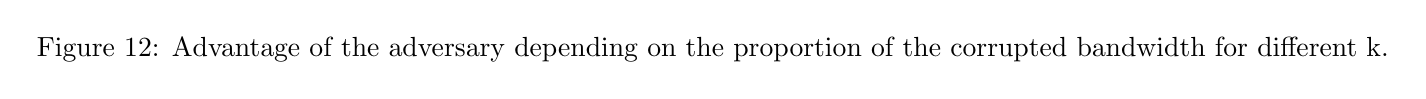
\begin{tikzpicture}
\node{Figure 12: Advantage of the adversary depending on the proportion of the corrupted bandwidth for different k.};
\end{tikzpicture}
\begin{tikzpicture}
\begin{axis}[
% axis lines=left,
xlabel={Proportion of the Corrupted Bandwidth},
ylabel={Advantage ($\advg$)},
width=8cm,
height=5cm,
xmin=0,
ymin=0,
legend style={at={(0.75,0.2)},
anchor=south},
legend cell align={left},
legend entries={$k = 10$,$k = 100$,$k = 1000$},
]

  \addplot[color=black,smooth,thick]
    table[col sep=comma,header=false,x index=0,y index=1]
    {data/lasthop_plot_bandwidth.csv};

  \addplot[color=blue,smooth,dashed,thick]
    table[col sep=comma,header=false,x index=0,y index=2]
    {data/lasthop_plot_bandwidth.csv};

  \addplot[color=red,only marks,mark=triangle*,mark size=3pt,fill=none]
    table[col sep=comma,header=false,x index=0,y index=1]
    {data/lasthop_plot_bandwidth_big_steps_1k.csv};
\end{axis}
\end{tikzpicture}

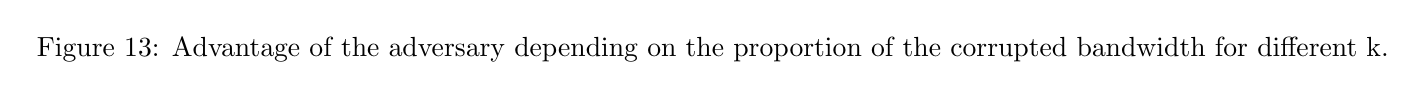
\begin{tikzpicture}
\node{Figure 13: Advantage of the adversary depending on the proportion of the corrupted bandwidth for different k.};
\end{tikzpicture}
  \begin{tikzpicture}
    \begin{axis}[
      % axis lines=left,
      xlabel={Share of the Corrupted Bandwidth},
      ylabel={Advantage ($\advg$)},
      width=8cm,
      height=5cm,
      xmin=0,
      ymin=0,
      legend style={at={(0.65,0.1)},
      anchor=south,nodes={scale=0.70, transform shape}},
      legend cell align={left},
      legend entries={Uniform with $\nmixes = 1\,000$,Bandwidth Based with $k = 100$},
    ]
    \addplot[color=blue,smooth,thick]
      table[col sep=comma,header=false,x index=0,y index=1]
      {data/lasthop_plot_proportion_1k.csv};
    \addplot[only marks,,mark size=3pt,mark=triangle*,fill=black]
      table[col sep=comma,header=false,x index=0,y index=1]
      {data/lasthop_plot_bandwidth_big_steps_100.csv};
    \end{axis}
   \end{tikzpicture}
\end{document}